\documentclass[utf8x, 12pt]{G7-32} 


% --------- -------- SETTINGS --------- --------

% --------- Настройки стиля ГОСТ 7-32 --------

% Гипертекстовое оглавление в PDF
\usepackage[
bookmarks=true, colorlinks=true, unicode=true,
urlcolor=black,linkcolor=black, anchorcolor=black,
citecolor=black, menucolor=black, filecolor=black,
]{hyperref}

\usepackage{graphicx}   % Пакет для включения рисунков
\DeclareGraphicsExtensions{.jpg,.pdf,.png}
\geometry{right=20mm}
\geometry{left=30mm}
\usepackage{enumerate}
\setcounter{tocdepth}{3} % Подробность оглавления


% --------- other settings --------
\usepackage{MnSymbol}
%\usepackage{simpsons}
% --------- -------- SETTINGS --------- --------



\begin{document}

\frontmatter 

% --------- -------- TITLE --------- --------

\begin{center} 

\large САНКТ-ПЕТЕРБУРГСИЙ ГОСУДАРСТВЕННЫЙ ПОЛИТЕХНИЧЕСКИЙ УНИВЕРСИТЕТ

\large Кафедра Компьютерных Систем и Программных Технологий \\[5.5cm] 

\huge ОТЧЕТ \\[0.6cm] % название работы, затем отступ 0,6см
\large по лабораторной работе №5\\
\large Тема: <<Инструмент тестов на проникновение Metaspoit>>\\
\large Дисциплина: <<Методы и средства защиты информации>>\\[3.7cm]

\end{center} 

\begin{flushright}
Выполнил: студент гр. 53501/2 \\
Пономарев М.A. \\[1.2cm]


Преподаватель \\
Вылегжанина К.Д.
\end{flushright}


\vfill 

\begin{center} 
\large Санкт-Петербург \\
2015
\end{center} 

\thispagestyle{empty}


% --------- -------- TITLE --------- --------

\thispagestyle{empty}
\setcounter{page}{0}
\tableofcontents
\clearpage
\mainmatter


\chapter{Задание}

\begin{enumerate}
	\item Подключиться к VNC-серверу, получить доступ к консоли
	\item Получить список директорий в общем доступе по протоколу SMB
	\item Получить консоль используя уязвимость в vsftpd
	\item Получить консоль используя уязвимость в irc
	\item Armitage Hail Mary
	\item Изучить три файла с исходным кодом эксплойтов или служебных скриптов на ruby и описать, что в них происходит
\end{enumerate}


\chapter{Выполнение}


\section{Подключиться к VNC-серверу, получить доступ к консоли}
\section{Получить список директорий в общем доступе по протоколу SMB}
\section{Получить консоль используя уязвимость в vsftpd}
\section{Получить консоль используя уязвимость в irc}
\section{Armitage Hail Mary}
\section{Изучить три файла с исходным кодом эксплойтов или служебных скриптов на ruby и описать, что в них происходит}


\begin{figure}[hhh!]
	\begin{center}
		%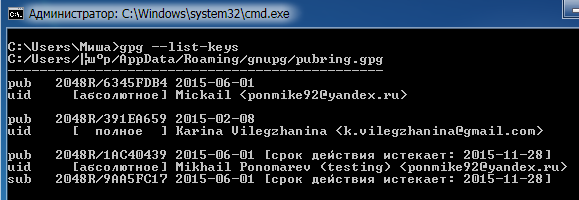
\includegraphics[width=12cm]{img/8_2}
	\end{center}
\end{figure}	


\end{document}
